\documentclass[11pt, a4paper, leqno]{article}
\usepackage{a4wide}
\usepackage[T1]{fontenc}
\usepackage[utf8]{inputenc}
\usepackage{float, afterpage, rotating, graphicx}
\usepackage{epstopdf}
\usepackage{longtable, booktabs, tabularx}
\usepackage{fancyvrb, moreverb, relsize}
\usepackage{eurosym, calc}
% \usepackage{chngcntr}
\usepackage{amsmath, amssymb, amsfonts, amsthm, bm}
\usepackage{caption}
\usepackage{mdwlist}
\usepackage{xfrac}
\usepackage{setspace}
\usepackage[dvipsnames]{xcolor}
\usepackage{subcaption}
\usepackage{minibox}
\usepackage{graphicx}
\graphicspath{{/bld/tables/}{/bld/graphs/}} % Specify the correct path for the missing image files

% \usepackage{pdf14} % Enable for Manuscriptcentral -- can't handle pdf 1.5
% \usepackage{endfloat} % Enable to move tables / figures to the end. Useful for some
% submissions.

\usepackage[
    natbib=true,
    bibencoding=inputenc,
    bibstyle=authoryear-ibid,
    citestyle=authoryear-comp,
    maxcitenames=3,
    maxbibnames=10,
    useprefix=false,
    sortcites=true,
    backend=biber
]{biblatex}
\AtBeginDocument{\toggletrue{blx@useprefix}}
\AtBeginBibliography{\togglefalse{blx@useprefix}}
\setlength{\bibitemsep}{1.5ex}
\addbibresource{refs.bib}

\usepackage[unicode=true]{hyperref}
\hypersetup{
    colorlinks=true,
    linkcolor=black,
    anchorcolor=black,
    citecolor=NavyBlue,
    filecolor=black,
    menucolor=black,
    runcolor=black,
    urlcolor=NavyBlue
}


\widowpenalty=10000
\clubpenalty=10000

\setlength{\parskip}{1ex}
\setlength{\parindent}{0ex}
\setstretch{1.5}


\begin{document}

\title{Does an increased risk of climate shocks affect individual resource extraction behaviour?
\thanks{Patricia Puspitasari, University of Bonn. Email: \ref{mailto:s75ppusp@uni-bonn.de}{\nolinkurl{s75ppusp [at] uni-bonn [dot] de}}.}}

\author{Patricia Puspitasari}

\date{
    {\bf Preliminary -- please do not quote}
    \\[1ex]
    \today
}

\maketitle


\begin{abstract}
    \input{sections/01Abstract}
\end{abstract}

\clearpage


\section{Experimental Procedure}\label{main:section3}
We conducted our lab experiment on January 2024 at the BonnEconLab to study the effect of climate shock on human extraction behaviour, particularly in the context of common pool resource. The experiment took place in three separate sessions, in each session 24 carefully selected participants took part in our lab experiment. Participants were chosen based on specific criteria: they had to be registered members of the BonnEconLab, proficient in German, and aged between 18 and 30 years. A crucial aspect of the selection process was also ensuring that these participants had not previously taken part in similar experiments. Since our study involves study with human subjects, our study has been pre-registered and approved for ethical review by the Institutional Review Board of the University of Bonn (Gesellschaft f\"ur experimentelle Wirtschaftsforschung (GfeW)) prior to conducting this experiment.

 Each of the three experimental session we conducted lasted approximately 45 minutes, and was divided into two main segments: a game followed by a comprehensive questionnaire, details of which are provided in the subsequent section. The design of our game segment follows the design of the forestry game by \citet{janssen2013breaking}.To build our instrument, we used O-tree, a Python-based software for experimental economic research\citet{chen2016otree}. No deception were done in our experiment, because complete instructions of the game were fully communicated through on screen display in the lab (see Appendix %\ref{app:A}).

 The game was divided into three parts: the baseline game as the control group, the anticipation treatments and the scarcity treatment. One part lasted five rounds, so the game lasted 15 rounds in total. Each participant played each part and was told in advance how many rounds the parts would last. Before the experiment began, each participant drew a number from 1 to 24 face down when they registered. This number indicated the participant’s cabin number for the experiment. We assigned the participants to groups of three depending on their cabin number, i.e. the participants with the numbers one to three were one group, the participants with the numbers four to six were one group and so on up to
24. During the experiment the participants were not permitted to communicate with each other, and
they were unaware of the group members to whom they had been assigned. The group assignments
remained fixed throughout the experiment.

All participants in each session of our study began by participating first in our Baseline game, followed by Anticipation game, Scarcity game and ended the experiment with a survey in which the order remain the same for all participants. Furthermore, in each game parts before participants began round 1 of each game, they were given a complete on screen instructions and subsequently asked to complete comprehension questions to ensure that participants fully understood the given instructions.


\section{Experimental Design}\label{main:section32}
The game segment in our experiment consists of 3 parts, namely Baseline game, Anticipation game and Scarcity game, where the last two are the treatments in our experiment. The baseline game is the standard forestry extraction game following \citet{janssen2013breaking}. The anticipation game follows a similar protocol to that in the baseline adjusted to a setting where there are risks of climate shock to occur and destroy the existing shared resources. In the scarcity game, subjects were put in a situation where the resource stock available is reduced significantly.

 We employed between and within subject design in our experiment game. Our within subject design is through the linear successions of the game parts, and between game design is employed under Anticipation game only, where subjects were randomly assigned to high or low probability group treatments. We designed the game as such in order to observe any behavioural changes that occurs between Baseline against the Anticipation game. By comparing the observed behavior between the two, we can observe how subject's behaviour might change in the presence of exogenous risk of climate shock. This risk presents uncertainty to the subjects individually and as a group, which consequently induces a lower expected value of the shared resource, providing incentives for subjects to harvest more now rather than later. Such design for the first two parts of our game will allow us to test our first hypothesis.

\medskip
\begin{adjustbox}{minipage=.7\textwidth,margin=0pt \smallskipamount,center}
    \itshape \noindent \textbf{H1}: An increased risk of climate shocks, that induces a lower expected future value of the resource, leads to an increase in harvest rates and a decrease in the stock of the resource.
\end{adjustbox}
\medskip

 Under the Anticipation part of the game, we randomly assigned subjects into 2 climate shock risk group, namely high and low probability. We designed it as such in order to see whether the relative size of the risk to occur has significant impact on subject's CPRs harvesting behaviour. With both groups experiencing elevated risk of climate shock, we can thus compare between the groups for observed behaviour changes.

 At the end of Anticipation game, groups may or may not experience actual climate shock. This differing random outcome allow us to further compare the results of Scarcity game where all subject restart a game but with only half of the resources they previously began the game with. Such setting is useful to compare whether subjects who have had prior experience of scarcity in the Anticipation game will behave differently from subjects who did not experience such scarcity when they later play our Scarcity game. However, we will not discuss our findings from this part in detail and will keep this for future studies.

 The survey within our laboratory experiment contains questions asking the participants regarding the optimum solution to the game, we adopted also questions from the short 24-item version of the Environmental Attitudes Inventory \cite{milfont2007} and the Global Preference Survey \cite{falk2018global}. The last two adopted survey questions are then used to measure personal attitude and perception towards environmentalism, and their preferences with respect to altruism, reciprocity, time preference, risk preference and trust. All these variables we believe to be important exogenous factors influencing individual and group extraction behaviour in the experiment, which led us to our second hypothesis.

\medskip
\begin{adjustbox}{minipage=.7\textwidth,margin=0pt \smallskipamount,center}
    \itshape \noindent \textbf{H2}: Subjects categorized as pro-environmental according to the Environmental Attitudes Inventory (EAI) extract less of the resource.
\end{adjustbox}
\medskip


    \subsection{Basline Game}\label{main:section32a}
    Our baseline forestry extraction game is designed to simulate a dynamic forestry resource. The initial number of forest resource consists of 100 trees. In each round, participants can take a maximum of seven trees from the forest resource. The baseline game lasts five rounds where participants can extract trees from the shared group forest in every round. After all members of the group have made their extraction decision, the total number of resource extracted will be deducted from the forest resource.

 The forest resource stock will regrow at 10\% rate in every round after extraction decision were made. For example, in the first round, given a total of 21 trees extracted, 79 trees remained in the forest. With the 10\% regrowth rate, 7.9 trees will then be added to the resource stock where the game will start in the second round with 86,9 trees. Despite the allowed regrowth rate, the forest stock cannot grow beyond its full capacity of 100 trees. We did not round down the number of trees regrown, but rather, allowed participants to only extract a fully grown tree represented by the integer numbers. Participants were also informed at the beginning of the experiment that for each trees extracted in each round, he or she will earn two points. Participants will also receive a one time payment of endowment in the amount of 50 points at the start of each game. However, this endowment is paid only once as a show up fee and does not influence the decision of participants throughout the game. Therefore, we will not include participants' endowment into the payoff function from here onwards.

 In addition to the trees harvested and the endowment, the participants were also told that the second element of their payoff will depend on the remaining number of trees left in the group's shared forest at the end of the 5$^{th}$ round after extraction and regrowth. These remaining trees will then double in value (4 points) and all group members will receive equal share of this value\footnote{see Appendix\ref{app:A} for detailed instructions of the experiment.}.


\paragraph{\textit{The Payoff Function.}}

Using game theoretical framework, the benchmark prediction on the standard individual extraction behaviour in our baseline game will depend on their payoff function. In the baseline game, the social payoff is the sum of individual group member \textit{i}'s payoff function. As a consequence both in group social payoff and individual payoff function will have \textbf{two} main components.

 The first component is their expected total individual payoff from harvesting the trees. Each individual $i$ in a group of 3 ($i \in \{1,2,3\}$) is allowed to extract $x$ number of trees at each round where $x \in \{0,1,2,3,4,5,6,7\}$, and each tree has a value of 2 points. With each game lasting 5 rounds, let $t\in \{1,2,3,4,5\}$ be the number of round this person is currently in. The expected total individual payoff from harvesting in all 5 rounds is then; $2\sum_{t=1}^{5}(x_{i,t})$. For each group consisting 3 individuals, the total harvest of a group in each round can be expressed as $X_{t} = \sum_{i=1}^{3} x_{i,t} $. Therefore, we can express the first component for each group's social payoff function as $2 \sum_{t=1}^{5} X_{t}$.

 The second component of the payoff function is the expected payoff from remaining trees in the forest at the end of the game (after regrowth in round 5). The remaining trees in the forest will depend on all player's extraction decision and the regrowth rate of $10\%$ in each round. In addition to that, the number of remaining trees in the forest cannot exceed 100 trees or fall below 0 at any given round. Thus, let $Z_t$ denote the number of trees that remained in the forest after harvesting and regrowth in a given round, where $0\leq Z_t \leq100$.

 In the first round of our baseline game every group began with 100 trees in their shared forest. Therefore, the remaining trees left in the first round can be expressed as $Z_{1}=(100-X_{1}) \times 1.1$. The second round remaining trees will then depend on remaining trees in round 1 and total number of trees extracted as a group. $Z_{2}$ is then defined as $Z_{2} = Z_{1} - X_{2} = (100-X_{1}) - X_{2}$. For subsequent rounds we follow the same pattern up until the last round, where $Z_5 = (Z_4 - X_5) 1.1$. This means that to find the remaining trees in the final round ($Z_5$) to determine individual and group expected social payoff from the remaining trees, we can define $Z_{5}$ as
\begin{equation}
\label{eq:1}
      Z_{5} = \left( \left( \left( \left( \left(100 - X_{1}\right) 1.1 - X_{2}\right) 1.1 - X_{3} \right) 1.1 - X_{4} \right) 1.1 - X_{5} \right) 1.1
\end{equation}
%where it simplifies to
%\begin{equation}
%\label{eq:2}
%    Z_{5} = 161.051 - 1.61051X_{1} - 1.4641X_{2} - 1.331X_{3} - 1.21X_{4} - 1.1X_{5}
%\end{equation}
%Combining equation (1) and (2) gives
%\begin{equation}
%\label{eq:3}
%    \pi_{i}=50+2\sum_{t=1}^{5} (x_{i,t})+\left( (161.051 - 1.61051X_{1} - 1.4641X_{2} - 1.331X_{3} - 1.21X_{4} - 1.1X_{5}) \times \frac{4}{3} \right)
%\end{equation}

\noindent Variable $Z_{5}$ defines the number of trees remained in a group's forest by the end of the 5$^{th}$ round and after the final regrowth rate. Each tree will be worth 4 points for the group, to be divided equally among three members of the group. The final part of each individual's payoff can then be expressed as $\frac{Z_{5} \times 4}{3}$. While the group payoff from trees that remained is $ \left(\frac{Z_{5} \times 4}{3}\right) \times 3 = Z_{5} \times {4}$.

\noindent Combining both payoff components, we have individual $i$'s payoff function with $i \in \{1,2,3\}$ as:
\begin{equation}
\label{eq:2}
    \pi_{i}=2\sum_{t=1}^{5} (x_{i,t})+\left( \frac{Z_{5} \times 4}{3} \right)
\end{equation}

\noindent And the group's payoff function as:
\begin{equation}
\label{eq:3}
    \Pi_{group} = \sum_{i=1}^{3} \pi_{i} = 2 \sum_{t=1}^{5} X_{t} + \left(Z_5 \times 4 \right)
\end{equation}


        \subsubsection{Behavioural Prediction in Baseline Game}\label{main:section32b}
        \input{sections/03.21Behavioural Prediction Baseline}

    \subsection{Anticipation Game}\label{main:section33a}
    %\documentclass[cprs.tex]{subfiles}
In the second part of our game, we focused on the anticipation effect of a climate shock. The purpose of this game is to investigate how individual extraction behaviour changes when the individual anticipates a potential climate shock and how this effect is amplified when there is an increased risk of climate shock to occur.

 To carry out the subsequent treatments, we placed the participants in a similar decision-making situation as in the Baseline game. Participants within a group remain the same and began the game with 100 trees in the shared forest. They may extract zero to seven trees per round. The difference to the baseline game is that, participants in a group were told that a climate shock might occur at the end of round five. In our game, a climate shock is framed in the context of a forest fire caused by drought and persistent heat, which destroys the trees in the shared forest. If a forest fire occurs at the end of the fifth round, the number of remaining trees will then be reduced by 50\% after the forest has regenerated. In order to observe the extent to which the subjects respond to an increased risk of a climate shock as described above, we created a between subject design in which we randomly assigned the groups equally into a high or a low probability shock group. The groups that were assigned to the high probability shock groups were told that they have 80\% chance of losing their remaining trees to a forest fire at the end of the game. The other half were assigned to the low probability group where they were told similar case but with only 20\% chance that a fire may occur.

\paragraph{\textit{The Payoff Function.}}

The payoff function under Anticipation game is similar to the Baseline game. The difference however is that the expected value of trees not harvested at the end of round five ($Z_5$) will no longer hold the same value of four as was in the previous game. Due to the presence of uncertainty, the expected value of the remaining trees changes according to the probability of forest fire occurring in a group's forest. Thus, individual expected payoff of those who were assigned to a high or low probability group can be expressed as
\begin{equation}
\label{eq:10}
    \pi_{i} = 2\sum_{t=1}^{5} (x_{i,t})+  Z_{5} \times 4 \left[ \dfrac{(0.5 \times p)+(1 \times 1-p)}{3} \right] \\
\end{equation}
And the group expected payoff adjusted to
\begin{equation}
\label{eq:11}
    \Pi_{group} = 2\sum_{t=1}^{5} (x_{i,t})+ Z_{5} \times 4 \left[ (0.5 \times p)+(1 \times 1-p) \right]
\end{equation}

 Table\ref{tab:7} summarizes the change in expected value from increased risk by calculating the expected value using the last term in equation\ref{eq:11}.

\begin{table}[htbp!]
  \centering
  \caption{Expected Value of Trees at the End of the Game by High and Low Probability Group}\label{tab:7}
  \begin{tabular}{p{0.2\linewidth} | p{0.2\linewidth} | p{0.15\linewidth} | p{0.35\linewidth}}
    \toprule
    \textbf{Group Type} & \textbf{Probability of Shock Occurring} & \textbf{\% Trees Remain} & \textbf{Expected Total Value of Each Tree Not Harvested} \\ %\midrule
    \multirow{2}{*}{\textbf{High}} & P(Shock)=0.8 & 50\% & \multirow{2}{*}{$ 4 \left[0.8(0.5)+(1-0.8)(1)\right]=2.4$} \\ \cline{2-3}
     & P(No Shock)=(1-0.8) & 100\%  \\ %\midrule
    \multirow{2}{*}{\textbf{Low}} & P(Shock)=0.2 & 50\% & \multirow{2}{*}{$ 4 \left[0.2(0.5)+(1-0.2)(1)\right]=3.6$} \\ \cline{2-3}
    & P(No Shock)=(1-0.2) & 100\%  \\
    \bottomrule
  \end{tabular}
\end{table}


%\noindent Given this change in expected value, the individual and group payoff function for high probability group are now defined as $\pi_{i}^{high}=2\sum_{t=1}^{5} (x_{i,t})+ \left( Z_{5} \times \frac{2.4}{3} \right)$, and $\Pi_{group}^{high}=2\sum_{t=1}^{5} (X_{t})+ \left( Z_{5} \times {2.4} \right)$ respectively. Similarly, the individual and group expected payoff function of those assigned to a low probability group can be expressed as $\pi_{i}^{low}=2\sum_{t=1}^{5} (x_{i,t})+ \left( Z_{5} \times \frac{3.6}{3} \right)$ and $\Pi_{group}^{low}=2\sum_{t=1}^{5} (X_{t})+ \left( Z_{5} \times {3.6} \right)$.

\noindent Given this change in expected value, the individual and group payoff function for high probability group are now defined as
\begin{equation}
\label{eq:4}
    \pi_{i}^{high}=2\sum_{t=1}^{5} (x_{i,t})+ \left( Z_{5} \times \frac{2.4}{3} \right)
\end{equation}
\begin{equation}
\label{eq:5}
    \Pi_{group}^{high}=2\sum_{t=1}^{5} (X_{t})+ \left( Z_{5} \times {2.4} \right)
\end{equation}

\noindent Similarly, the individual and group expected payoff function of those assigned to a low probability group can be expressed as
\begin{equation}
\label{eq:6}
    \pi_{i}^{low}=2\sum_{t=1}^{5} (x_{i,t})+ \left( Z_{5} \times \frac{3.6}{3} \right)
\end{equation}
\begin{equation}
\label{eq:7}
    \Pi_{group}^{low}=2\sum_{t=1}^{5} (X_{t})+ \left( Z_{5} \times {3.6} \right)
\end{equation}

 Following the baseline game, the number of trees remained in the forest at the end of the game ($Z_{5}$) depends on the previous rounds extraction decision and the 10\% regrowth rate. This potential 50\% drop in social payoff reduces their expected future value. The increase in uncertainty of their social payoff provides an incentive for participants to extract more earlier in the game to gain payoff for themselves now rather than uncertain outcome in the future.


        \subsubsection{Behavioural Prediction in Anticipation Game}\label{main:section33b}
        \paragraph{\textit{Nash equilibrium and the cooperative solution.}}
The Nash equilibrium under Anticipation game also remain as in the Baseline game. We can expect a fully rational and selfish agent to always harvest seven trees at any given round to maximize his or her individual payoff as defined in equation \ref{eq:6} and \ref{eq:7}. Similarly, the Pareto optimum solution for cooperative equilibrium under Anticipation Game is also the same as in the baseline. The difference is that, in Table \ref{tab:7} under Anticipation Game, the expected value of every tree at the end of the game is now lower than four points yet remains higher than the two points participants could receive from harvesting. This means that the same socially optimum strategy persists. Except now, this increased risk causes cooperative solution to be more unstable than in the previous game to maintain. This instability arises from the fact that the decrease in future expected value per trees for society provides even more incentives for agents to harvest now rather than leaving the chance to lose out on the value that they could have received by harvesting now.
 \begin{figure}[H]
  \centering
  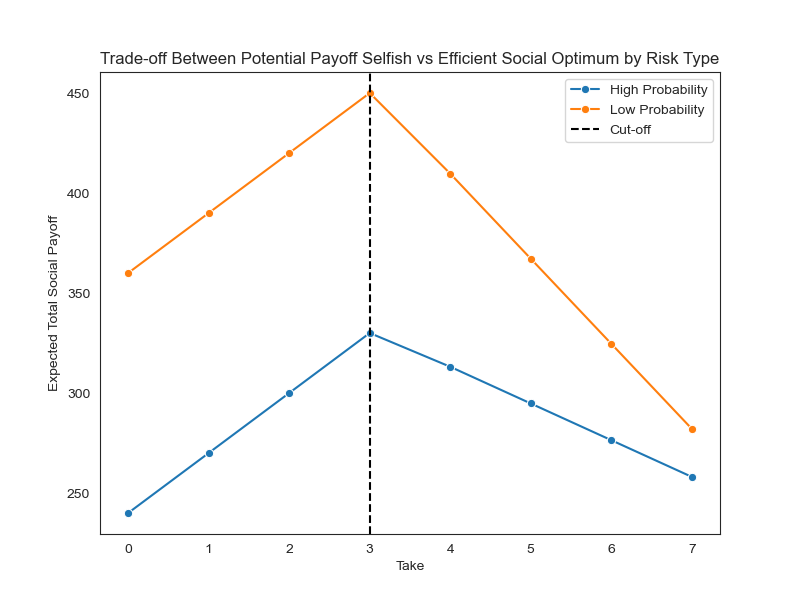
\includegraphics[width=0.6\linewidth]{../bld/graphs/0.Tradeoff2.png}
  \caption{Trade-off Between Potential Payoff Selfish vs Efficient Social Optimum}
  \label{fig:tradeoff3}
\end{figure}
 \paragraph{\textit{Expected Behaviour.}}

 Figure \ref{fig:tradeoff3} illustrates the cooperative equilibrium and the trade-off between efficiency and selfish behaviour. For any symmetric strategy that harvest any amount less than three trees is not optimal even though it is socially beneficial for everyone. Similarly, any symmetric strategy that harvest more than three trees is also not socially beneficial for everyone due to agents' selfish behaviour that strive to benefit own payoff at the expense of society. Notice that although there is an increased risk, the predicted behaviour and types do not change between Baseline and the Anticipation game as illustrated in Figure \ref{fig:tradeoff2} and \ref{fig:tradeoff3}.


    \subsection{Scarcity Game}\label{main:section34a}
    In the third part of our experiment, we investigated the extent to which an experienced climate shock in the past influenced our participants in their extraction behaviour. To observe this scarcity effect we employed a within subject design. The participants were asked to make extraction decision as part of a group of three similar to the previous games. The main difference here is that in the Anticipation game, participants assigned to high or low probability shock groups may or may not experience shock at the end of the 5$^{th}$ round. The key treatment in the game is that, some participants did not experience climate shock, yet some did (see Table \ref{tab:2} for subject and group treatment allocation).

\noindent The purpose of this game is thus to see whether participants (and groups) with prior experience of scarcity due to forest fire will behave differently to those who have not experienced a climate shock before. To create a scarcity situation, participants were told that they will start this game with only 50 trees (50\% of baseline initial forest stock to mimic the condition set in the Anticipation game) instead of 100 trees. Additionally, the individual harvest restriction per round now depended on the number of trees in the forest as presented in Table \ref{tab:1}. Although each group began with a shared forest stock of 50 trees, group's shared forest may regrow beyond the initial 50 trees up to the maximum 100 trees. Thus, should the group chose to refrain from extracting beyond the growth rate of 10\% - that is less than 5 trees), the forest stock can regrow almost to its full capacity of 100 trees. Given that there is no uncertainty of another shock to occur, there is an incentive for participants in a group to maximize their individual payoff by maximizing the number or their shared forest resource.

\begin{table}[htbp!]
  \centering
  \caption{Maximum harvest table.}\label{tab:1}
  \begin{tabular}{ll}
    \toprule
    Number of trees in forest resource & Maximum allowable harvest \\
    \midrule
    21-100 & 7 \\
    18-20 & 6  \\
    15-17 & 5 \\
    12-14 & 4 \\
    9-11 & 3 \\
    6-8 & 2 \\
    3-5 & 1 \\
    0-2 & 0 \\
    \bottomrule
  \end{tabular}
\end{table}


\paragraph{\textit{The Payoff Function.}} The payoff function of individual and group under our scarcity game remain the same as in equation \eqref{eq:1}. The only difference if the number of starting trees in round 1 which affects the number of remaining trees left in the forest which in turn affects social payoff. Thus, we can reiterate $Z_{5}$ as
\begin{equation}
\label{eq:8}
    Z_{5} = \left( \left( \left( \left( \left(50 - X_{1}\right) 1.1 - X_{2}\right) 1.1 - X_{3} \right) 1.1 - X_{4} \right) 1.1 - X_{5} \right) 1.1
\end{equation}
%where it simplifies to
%\begin{equation}
%\label{eq:9}
%    Z_{5} = 80.5255 - 1.61051X_{1} - 1.4641X_{2} - 1.331X_{3} - 1.21X_{4} - 1.1X_{5}
%\end{equation}

\noindent Although the definition of $Z_5$ changes under scarcity game, the payoff function for individual and group remains the same as in the ones under baseline game defined in equation \ref{eq:2} for individual payoff function and \ref{eq:3} for group payoff function.

\noindent We re-write individual payoff function again below:
\begin{equation*}
    \pi_{i}=2\sum_{t=1}^{5} (x_{i,t})+\left( \frac{Z_{5} \times 4}{3} \right)
\end{equation*}

\noindent And the group's payoff function:
\begin{equation*}
    \Pi_{group} = \sum_{i=1}^{3} \pi_{i} = 2 \sum_{t=1}^{5} X_{t} + \left(Z_5 \times 4 \right)
\end{equation*}


        \subsubsection{Behavioural Prediction in Scarcity Game}\label{main:section34b}
        In the third part of our experiment, we investigated the extent to which an experienced climate shock in the past influenced our participants in their extraction behaviour. To observe this scarcity effect we employed a within subject design. The participants were asked to make extraction decision as part of a group of three similar to the previous games. The main difference here is that in the Anticipation game, participants assigned to high or low probability shock groups may or may not experience shock at the end of the 5$^{th}$ round. The key treatment in the game is that, some participants did not experience climate shock, yet some did (see Table \ref{tab:2} for subject and group treatment allocation).

\noindent The purpose of this game is thus to see whether participants (and groups) with prior experience of scarcity due to forest fire will behave differently to those who have not experienced a climate shock before. To create a scarcity situation, participants were told that they will start this game with only 50 trees (50\% of baseline initial forest stock to mimic the condition set in the Anticipation game) instead of 100 trees. Additionally, the individual harvest restriction per round now depended on the number of trees in the forest as presented in Table \ref{tab:1}. Although each group began with a shared forest stock of 50 trees, group's shared forest may regrow beyond the initial 50 trees up to the maximum 100 trees. Thus, should the group chose to refrain from extracting beyond the growth rate of 10\% - that is less than 5 trees), the forest stock can regrow almost to its full capacity of 100 trees. Given that there is no uncertainty of another shock to occur, there is an incentive for participants in a group to maximize their individual payoff by maximizing the number or their shared forest resource.

\begin{table}[htbp!]
  \centering
  \caption{Maximum harvest table.}\label{tab:1}
  \begin{tabular}{ll}
    \toprule
    Number of trees in forest resource & Maximum allowable harvest \\
    \midrule
    21-100 & 7 \\
    18-20 & 6  \\
    15-17 & 5 \\
    12-14 & 4 \\
    9-11 & 3 \\
    6-8 & 2 \\
    3-5 & 1 \\
    0-2 & 0 \\
    \bottomrule
  \end{tabular}
\end{table}


\paragraph{\textit{The Payoff Function.}} The payoff function of individual and group under our scarcity game remain the same as in equation \eqref{eq:1}. The only difference if the number of starting trees in round 1 which affects the number of remaining trees left in the forest which in turn affects social payoff. Thus, we can reiterate $Z_{5}$ as
\begin{equation}
\label{eq:8}
    Z_{5} = \left( \left( \left( \left( \left(50 - X_{1}\right) 1.1 - X_{2}\right) 1.1 - X_{3} \right) 1.1 - X_{4} \right) 1.1 - X_{5} \right) 1.1
\end{equation}
%where it simplifies to
%\begin{equation}
%\label{eq:9}
%    Z_{5} = 80.5255 - 1.61051X_{1} - 1.4641X_{2} - 1.331X_{3} - 1.21X_{4} - 1.1X_{5}
%\end{equation}

\noindent Although the definition of $Z_5$ changes under scarcity game, the payoff function for individual and group remains the same as in the ones under baseline game defined in equation \ref{eq:2} for individual payoff function and \ref{eq:3} for group payoff function.

\noindent We re-write individual payoff function again below:
\begin{equation*}
    \pi_{i}=2\sum_{t=1}^{5} (x_{i,t})+\left( \frac{Z_{5} \times 4}{3} \right)
\end{equation*}

\noindent And the group's payoff function:
\begin{equation*}
    \Pi_{group} = \sum_{i=1}^{3} \pi_{i} = 2 \sum_{t=1}^{5} X_{t} + \left(Z_5 \times 4 \right)
\end{equation*}


\section{Descriptive Statistics}\label{main:section41}
\subfile{sections/04.1 Descriptive Statistics}
\section{Results}\label{main:section42}
\subfile{sections/04.2Lab Subjects Results}
If you are using this template, please cite this item from the references:
%\citet{GaudeckerEconProjectTemplates}. CHECK IF THIS COMES OUT


% section introduction (end)



\setstretch{1}
\printbibliography
\setstretch{1.5}


 \appendix
 \section{Appendix D - Lab Experiment Instructions}\label{app:A}
 \vspace{15pt}
 \subsection{Welcome Page}
 \subfile{sections/06.A1 Welcome Page}

     \subsection{Instructions for Baseline Game}
     \subfile{sections/06.A2 Baseline Instructions}

     \subsection{Example}
     \subfile{sections/06.A3 Example Page}

     \subsection{Instructions for Anticipation Game}
     \subfile{sections/06.A4 Anticipation Instruction}

     \subsection{Instructions for Scarcity Game}
     \subfile{sections/06.A5 Scarcity Instructions}

% The chngctr package is needed for the following lines.
 \counterwithin{table}{section}
 \counterwithin{figure}{section}

\end{document}
